\documentclass[letterpaper,10pt,titlepage,draftclsnofoot,onecolumn,onesided] {IEEEtran}
\usepackage{listings}
\usepackage{underscore}
\usepackage[bookmarks=true]{hyperref}
\usepackage[utf8]{inputenc}
\usepackage[english]{babel}
\usepackage{titling}
\usepackage{graphicx}
\usepackage[noadjust]{cite}
\nocite{*}
\graphicspath{ {img/} }
\usepackage{abstract}

% C: I added this package for the definitions portion of the document
\usepackage{amsthm}

\newcommand{\namesigdate}[2][4cm]{%
  \begin{tabular}{@{}p{#1}@{}}
    #2 \\[2\normalbaselineskip] \hrule \\[0pt]
    {\small \textit{Signature}} \\[2\normalbaselineskip] \hrule \\[0pt]
    {\small \textit{Date}}
  \end{tabular}
}
\newcommand{\studentnamesigdate}[2][4cm]{%
  \begin{tabular}{@{}p{#1}@{}}
    #2 \\[2\normalbaselineskip] \hrule \\[0pt]
    {\small \textit{Signature}} \\[2\normalbaselineskip] \hrule \\[0pt]
    {\small \textit{Signature}} \\[2\normalbaselineskip] \hrule \\[0pt]
    {\small \textit{Signature}} \\[2\normalbaselineskip] \hrule \\[0pt]
    {\small \textit{Signature}} \\[2\normalbaselineskip] \hrule \\[0pt]
    {\small \textit{Date}}
  \end{tabular}
}

\hypersetup{
    bookmarks=false,    % show bookmarks bar?
    pdftitle={Progress Report},    % title
    pdfauthor={Cramer Smith, Sam Lichlyter, Eric Winkler, Zach Schneider},                     % author
    pdfsubject={Progress Report},                        % subject of the document
    pdfkeywords={IFT, Report, Postal}, % list of keywords
    colorlinks=true,       % false: boxed links; true: colored links
    linkcolor=black,       % color of internal links
    citecolor=black,       % color of links to bibliography
    filecolor=black,        % color of file links
    urlcolor=blue,        % color of external links
    linktoc=page            % only page is linked
} 

% Document Title:
\def\doctitle{A Tool to Automatically Organize the Structure of a Codebase Using Information Foraging Theory Design Patterns}
\def\doctype{Progress Report}
\def\team{Team Postal | Group \#38}

\markboth{Oregon State University}{\doctitle}

\begin{document}

\title{\Huge{\bfseries{\textsf{\doctitle}}}\\\textsf{\Large{\doctype}}\\\textsf{\large{\team}}}
\author{Cramer Smith, Sam Lichlyter, Eric Winkler, Zach Schneider}

\maketitle
\vfill

\vfill

\pagebreak

\tableofcontents

\pagebreak


\pagebreak

\section{Project Purpose and Goals}
Developer tools are often complex pieces of software. 
Gathering and manipulating useful information for a programmer can often be a slow and costly process. 
By implementing Information Foraging Theory design patterns in the creation of these tools, the information collected may be more useful or obtained faster. 
Information Foraging Theory (IFT) is the theory and math behind the choices people make to maximize the value of the information they find versus the cost of getting that information.
The aim of this project is to develop a tool that will act as a proof of concept for IFT and increase developer efficiency.

The Postal extension is being designed to allow developers to more quickly search through and better visualize their projects.
This extension will also help developers create clearer and cleaner code structure by offering reminders and suggestions about the best coding practices in the programming language they are currently using.
Any major errors or incompatibilities within the project or its files will be reported to the developer as well.


\section{Current Status}
\subsection{Parsers}
The current implementation of the extension has one parser which parses HTML.
This parser is implemented in Perl using the Simple TokeParser which looks for specific tags and a specific attribute from that tag.
For example, this HTML parser specifically looks for the anchor (\verb|a|) tag and the hyperlink reference (\verb|href|) attribute and returns those values which are the links to either outside websites or internal pages.

\subsection{User Interface}
The user interface is currently running off of dummy, static data. 
It opens up in a new window using a program called Electron as opposed to a web browser to cut down on the overhead associated with all the complexities of the web browser.
It shows each web page as a node and each link from one page to another as an edge in a graph. See Figure 1.
\begin{figure}
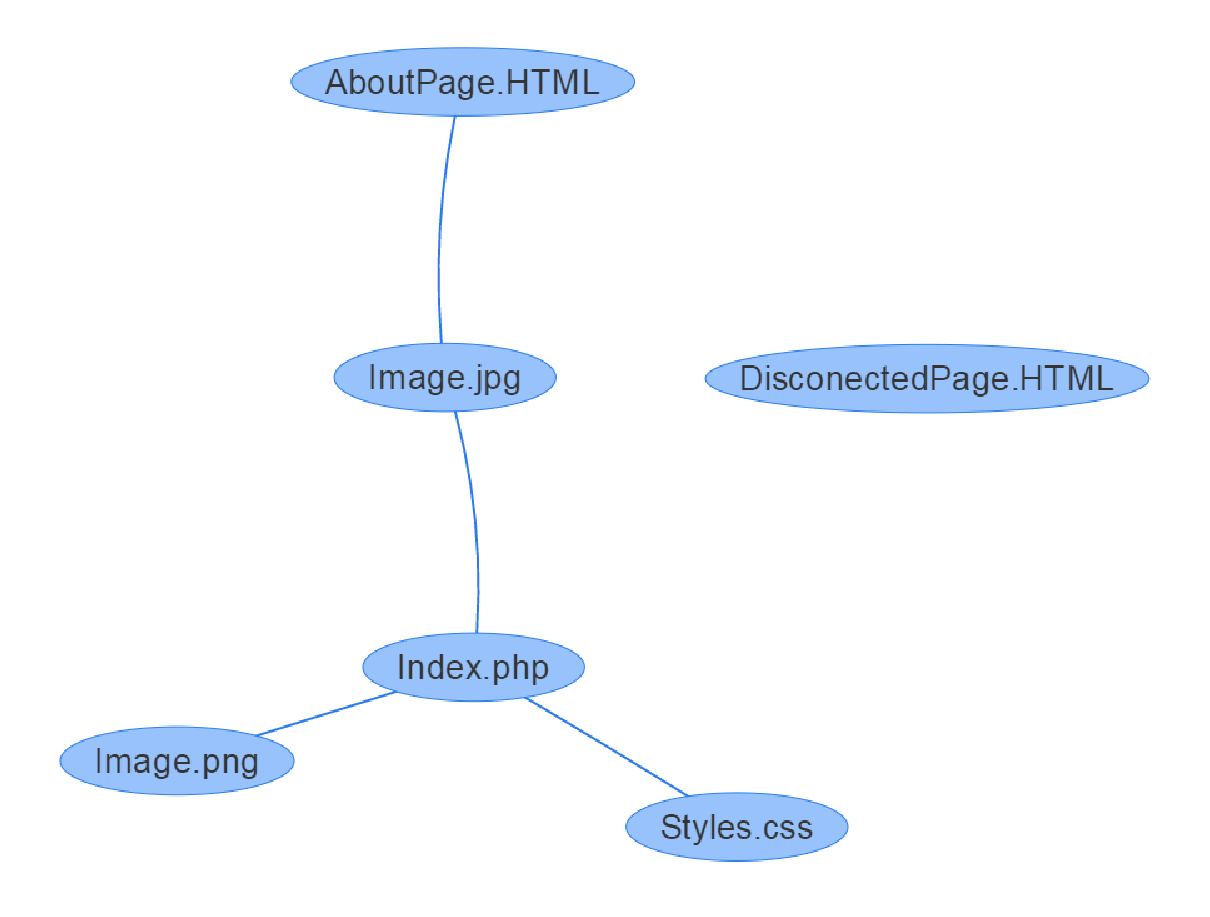
\includegraphics[width=300px]{UIMockupEPS}
\caption{User Interface Example}
\end{figure}

\subsection{Data Layer}


\section{Problems and Solutions}
	\subsection{Pre-Week 3}

	\subsection{Week 3}

	\subsection{Week 4}

	\subsection{Week 5}

	\subsection{Week 6}

	\subsection{Week 7}

	\subsection{Week 8}

	\subsection{Week 9}

	\subsection{Week 10}

\section{Prototype Code Samples}
	
	\subsection{FileMap UI}
	\begin{lstlisting}

	\end{lstlisting}

	\subsection{HTML Parser}
	\begin{lstlisting}

	\end{lstlisting}

\section{Fall Term Retrospective}
	\begin{center}
		\begin{tabular}{ |  p{0.25\linewidth}  |  p{0.25\linewidth}  | p{0.25\linewidth} | p{0.25\linewidth} |}
		\hline
		Topic & Positives & Deltas & Actions \\ \hline
		
			Communication with client 
		& 
			\begin{itemize}
				\item Flexible in terms of project requirements.
				\item Provided the team with a mock up application architecture.
				\item Easy to work with.
			\end{itemize}
		& 
			\begin{itemize}
				\item Frequency and clarity of communication need to be improved.
			\end{itemize}
		&
			\begin{itemize}
				\item Solidify team member responsibilities (Sam is in charge of emailing the client).
				\item The team as a whole will need to make sure Sam is aware of things that need to be communicated with the client.
			\end{itemize} 
		\\ \hline
			Team Effectiveness 
		& 
			\begin{itemize}
				\item Members have flexible schedules and are easy to sit down with.
				\item Members all do a good job of quickly replying to communications.
				\item Members have a positive attitude.
			\end{itemize}
		& 
			\begin{itemize}
				\item As a team, assignments do not get much planning and are usually done last minute.
				\item There is no clear team leader.
			\end{itemize}
		&
			\begin{itemize}
				\item Assign a pseudo team leader with the responsibility of tracking/ scheduling tasks and work assignments.
			\end{itemize} 
		\\ \hline
			Implementation 
		& 
			\begin{itemize}
				\item The team has become much more capable at developing with the VSC IDE.
				\item The Team has already built a couple of working prototypes for the client.
			\end{itemize}
		& 
			\begin{itemize}
				\item The Gantt chart is currently out of date and needs updating.
				\item Some technical implantation obstacles have yet to be addressed (npm auto installing).
			\end{itemize}
		&
			\begin{itemize}
				\item Update Gantt chart to better reflect the current progress and set new goal deadlines for winter term.
			\end{itemize} 
		\\ \hline
			Design 
		& 
			\begin{itemize}
				\item The current design meets requirements and team members are aware of their design related responsibilities.
			\end{itemize}
		& 
			\begin{itemize}
				\item IFT Design Pattern tie-ins are not 100\% clear and as a major requirement of the project, they need to be.
				\item Parse needs to be redesigned to better match our scope. See Week 10 notes.
			\end{itemize}
		&
			\begin{itemize}
				\item The team will need to meet to re-design the parser component of the extension and review the selected IFT design patterns.
			\end{itemize} 
		\\ \hline
			Documentation 
		& 
			\begin{itemize}
				\item All assigned documentation is currently in a workable state.
			\end{itemize}
		& 
			\begin{itemize}
				\item Team members feel that the documentation is typically rushed and not a descriptive as it should be.
				\item Team members have a difficult time interpreting the IEEE standards and thi may be a partial cause to the above.
			\end{itemize}
		&
			\begin{itemize}
				\item A team member will take a leadership position to schedule work tasks which will ensure that the team has sufficient time to complete the documentation assignments to a higher standard. 
			\end{itemize} 
		\\ \hline
		\end{tabular}
	\end{center}


\pagebreak
\bibliographystyle{IEEEtran}
\bibliography{progress}
\pagebreak

\namesigdate{Client Signature} \hfill 
\studentnamesigdate[4cm]{Student Signatures}
\end{document}
